\clearpage
\appendix
\chapter{Additional Evaluation Results}

This chapter includes figures showing additional evaluation results described in \Cref{subsec:eval.quant} and \Cref{subsec:eval.qual}.

\clearpage
\section{Quantitative Evaluation}

\begin{figure}[!h]
    \centering
    \begin{subfigure}{.3\textwidth}
    \centering
    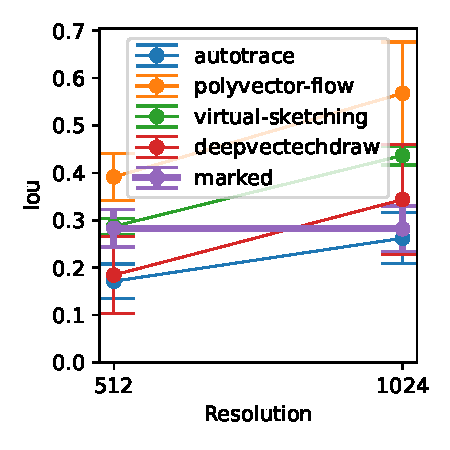
\includegraphics[width=\textwidth]{graphics/eval/iou_1024-1.024_True_tonari.pdf}
    \caption{The average \gls{iou}.}
\end{subfigure}
    \begin{subfigure}{.3\textwidth}
    \centering
    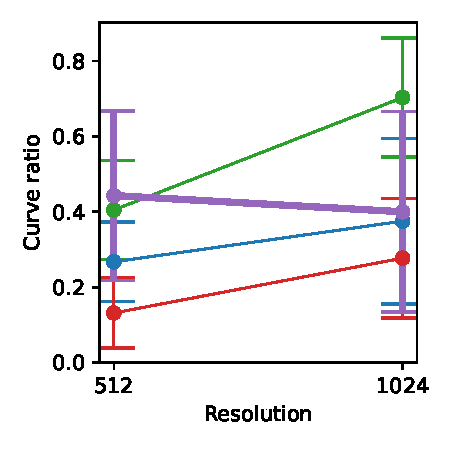
\includegraphics[width=\textwidth]{graphics/eval/curve ratio_1024-1.024_True_tonari.pdf}
    \caption{The average curve ratio.}
\end{subfigure}
    \begin{subfigure}{.3\textwidth}
    \centering
    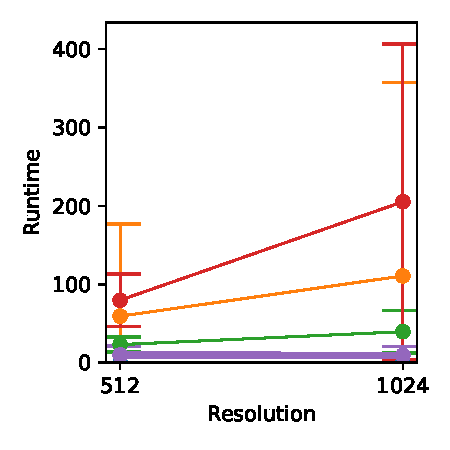
\includegraphics[width=\textwidth]{graphics/eval/runtime_1024-1.024_True_tonari.pdf}
    \caption{The average runtime.}
\end{subfigure}
    \begin{subfigure}{.3\textwidth}
    \centering
    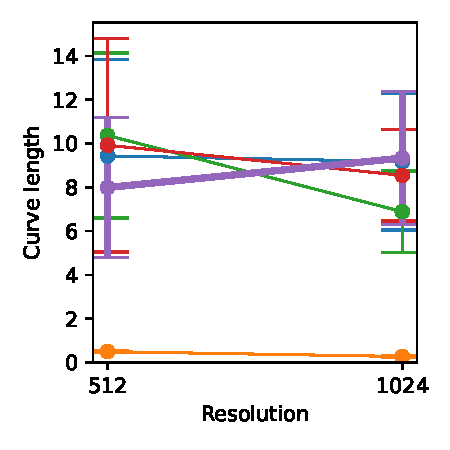
\includegraphics[width=\textwidth]{graphics/eval/curve length_1024-1.024_True_tonari.pdf}
    \caption{The average curve length.}
\end{subfigure}
    \begin{subfigure}{.3\textwidth}
    \centering
    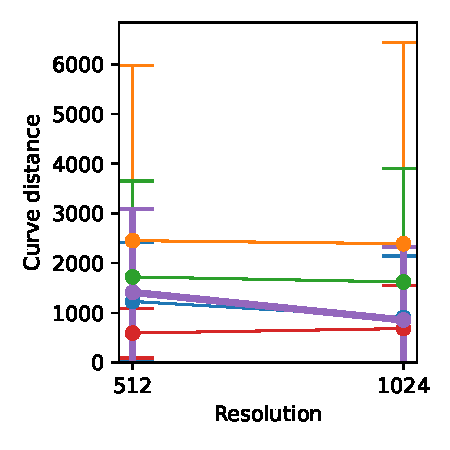
\includegraphics[width=\textwidth]{graphics/eval/curve distance_1024-1.024_True_tonari.pdf}
    \caption{The total curve distance.}
\end{subfigure}
    \begin{subfigure}{.3\textwidth}
    \centering
    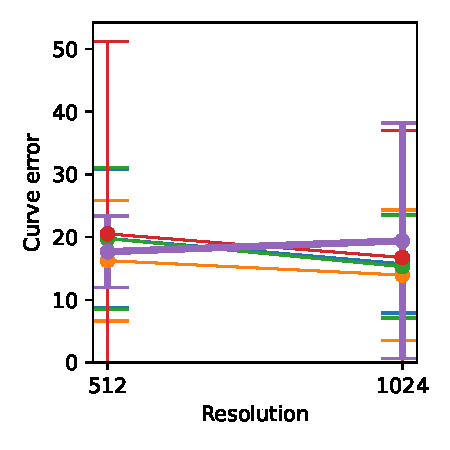
\includegraphics[width=\textwidth]{graphics/eval/curve error_1024-1.024_True_tonari.pdf}
    \caption{The average curve error.}
\end{subfigure}
    \caption{Metrics for the line-art image vectorization methods evaluated on binarized images with 512px and 1024px resolution, respectively. Points denote the median of the metric, while vertical bars denote the \gls{iqr}. Horizontal lines show the trend of the metric. The metrics for the method developed in this work are emphasized. Note that they are not significantly affected by the image resolution even if they are binarized.}
    \label{fig:metric_1024_True_tonari}
\end{figure}

\begin{figure}[h]
    \centering
    \begin{subfigure}{.3\textwidth}
    \centering
    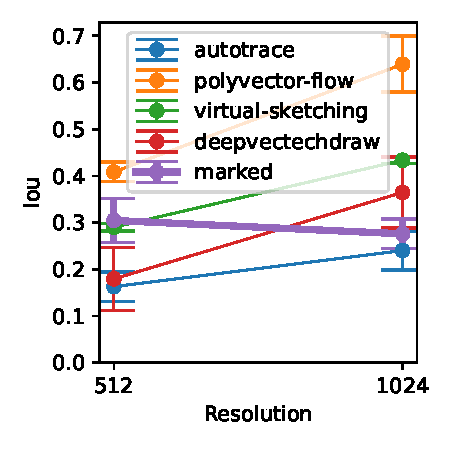
\includegraphics[width=\textwidth]{graphics/eval/iou_1024-1.024_True_sketchbench.pdf}
    \caption{The average \gls{iou}.}
\end{subfigure}
    \begin{subfigure}{.3\textwidth}
    \centering
    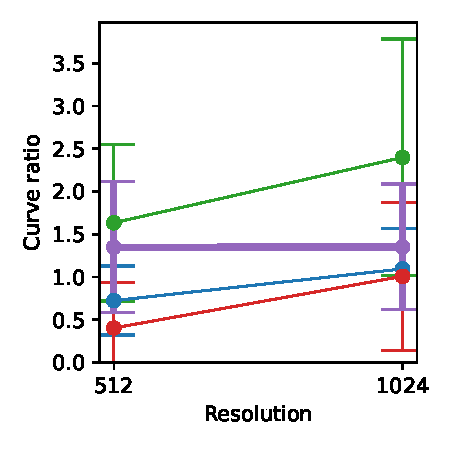
\includegraphics[width=\textwidth]{graphics/eval/curve ratio_1024-1.024_True_sketchbench.pdf}
    \caption{The average curve ratio.}
\end{subfigure}
    \begin{subfigure}{.3\textwidth}
    \centering
    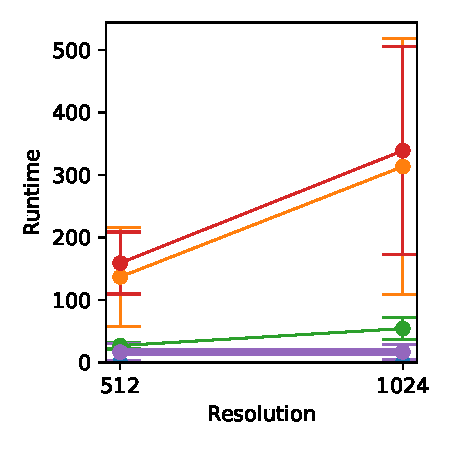
\includegraphics[width=\textwidth]{graphics/eval/runtime_1024-1.024_True_sketchbench.pdf}
    \caption{The average runtime.}
\end{subfigure}
    \begin{subfigure}{.3\textwidth}
    \centering
    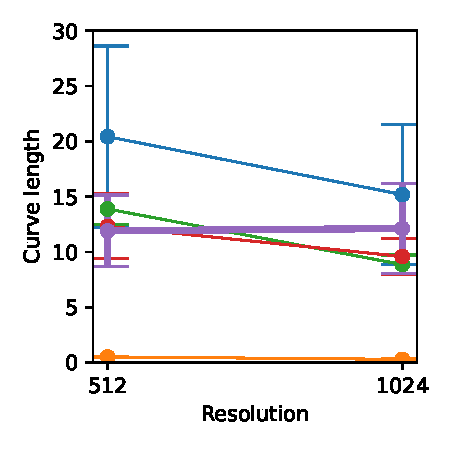
\includegraphics[width=\textwidth]{graphics/eval/curve length_1024-1.024_True_sketchbench.pdf}
    \caption{The average curve length.}
\end{subfigure}
    \begin{subfigure}{.3\textwidth}
    \centering
    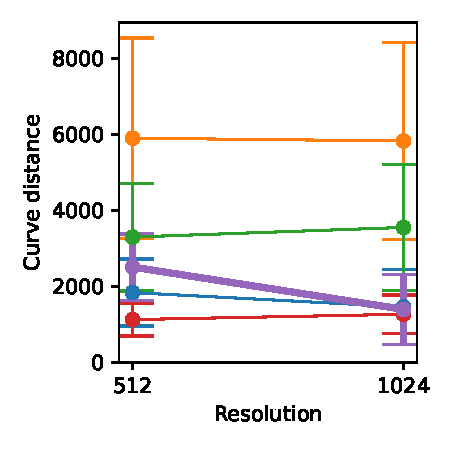
\includegraphics[width=\textwidth]{graphics/eval/curve distance_1024-1.024_True_sketchbench.pdf}
    \caption{The total curve distance.}
\end{subfigure}
    \begin{subfigure}{.3\textwidth}
    \centering
    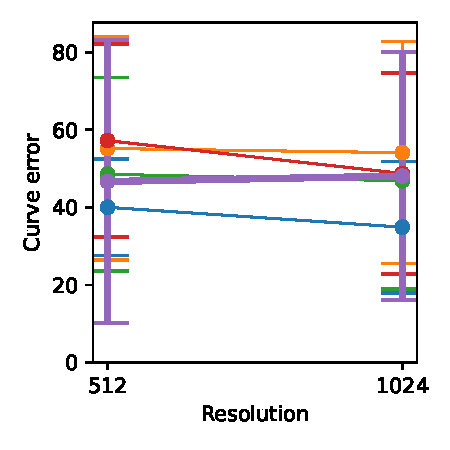
\includegraphics[width=\textwidth]{graphics/eval/curve error_1024-1.024_True_sketchbench.pdf}
    \caption{The average curve error.}
\end{subfigure}
    \caption{The same comparison as in \Cref{fig:metric_1024_True_tonari} on the SketchBench test dataset instead of the Tonari test dataset.}
    \label{fig:metric_1024_True_sketchbench}
\end{figure}

\begin{figure}[h]
    \centering
    \begin{subfigure}{.3\textwidth}
    \centering
    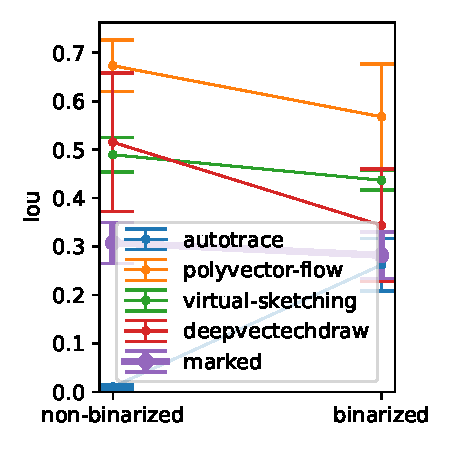
\includegraphics[width=\textwidth]{graphics/eval/iou_True_1024-1.024_tonari.pdf}
    \caption{The average \gls{iou}.}
\end{subfigure}
    \begin{subfigure}{.3\textwidth}
    \centering
    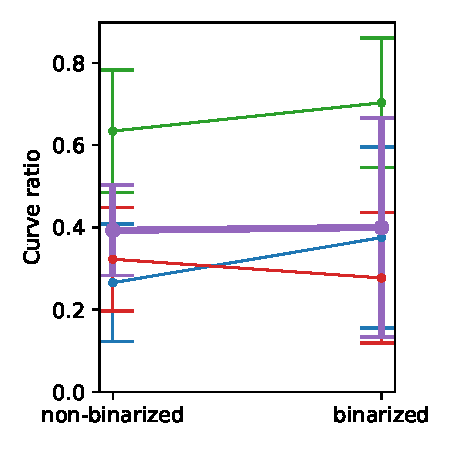
\includegraphics[width=\textwidth]{graphics/eval/curve ratio_True_1024-1.024_tonari.pdf}
    \caption{The average curve ratio.}
\end{subfigure}
    \begin{subfigure}{.3\textwidth}
    \centering
    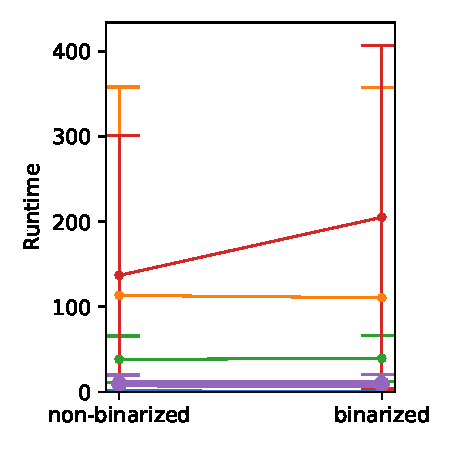
\includegraphics[width=\textwidth]{graphics/eval/runtime_True_1024-1.024_tonari.pdf}
    \caption{The average runtime.}
\end{subfigure}
    \begin{subfigure}{.3\textwidth}
    \centering
    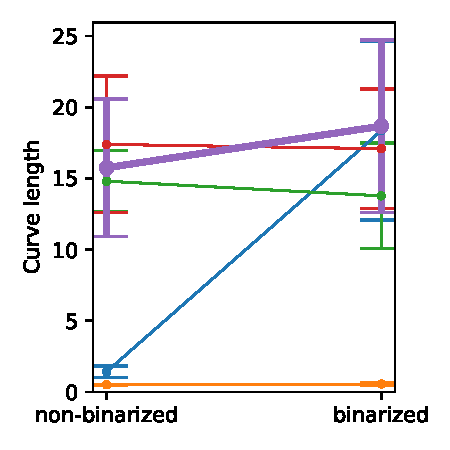
\includegraphics[width=\textwidth]{graphics/eval/curve length_True_1024-1.024_tonari.pdf}
    \caption{The average curve length.}
\end{subfigure}
    \begin{subfigure}{.3\textwidth}
    \centering
    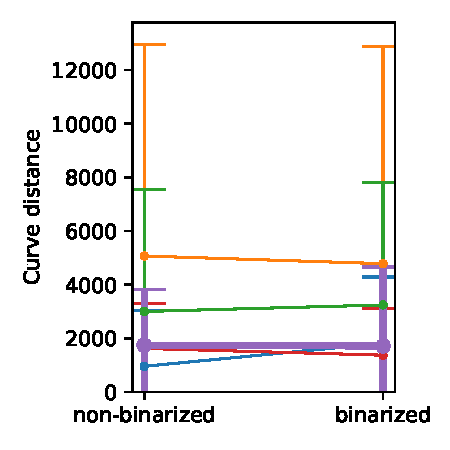
\includegraphics[width=\textwidth]{graphics/eval/curve distance_True_1024-1.024_tonari.pdf}
    \caption{The total curve distance.}
\end{subfigure}
    \begin{subfigure}{.3\textwidth}
    \centering
    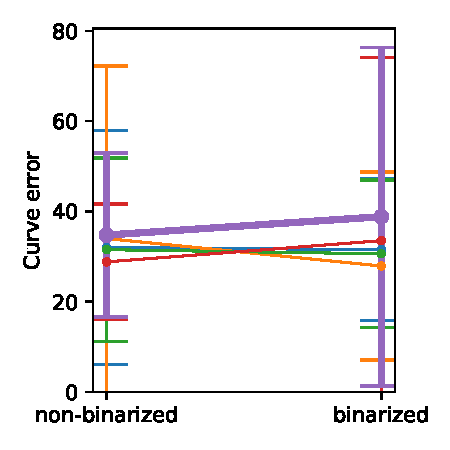
\includegraphics[width=\textwidth]{graphics/eval/curve error_True_1024-1.024_tonari.pdf}
    \caption{The average curve error.}
\end{subfigure}
    \caption{Metrics for the line-art image vectorization methods evaluated on binarized and non-binarized images with 1024px resolution, respectively. Points denote the median of the metric, while vertical bars denote the \gls{iqr}. The metrics for the method developed in this work are emphasized. Note that they are not significantly affected by binarization even on high-resolution images.}
    \label{fig:metric_True_1024_tonari}
\end{figure}

\begin{figure}[h]
    \centering
    \begin{subfigure}{.3\textwidth}
    \centering
    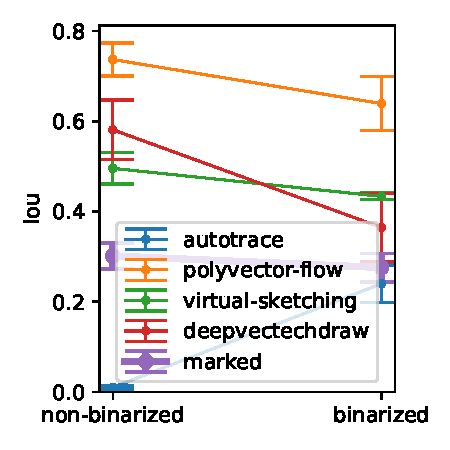
\includegraphics[width=\textwidth]{graphics/eval/iou_True_1024-1.024_sketchbench.pdf}
    \caption{The average \gls{iou}.}
\end{subfigure}
    \begin{subfigure}{.3\textwidth}
    \centering
    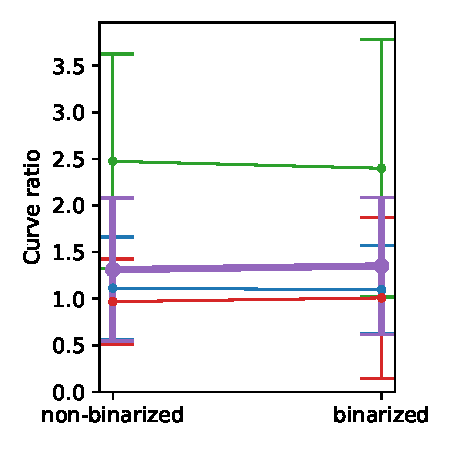
\includegraphics[width=\textwidth]{graphics/eval/curve ratio_True_1024-1.024_sketchbench.pdf}
    \caption{The average curve ratio.}
\end{subfigure}
    \begin{subfigure}{.3\textwidth}
    \centering
    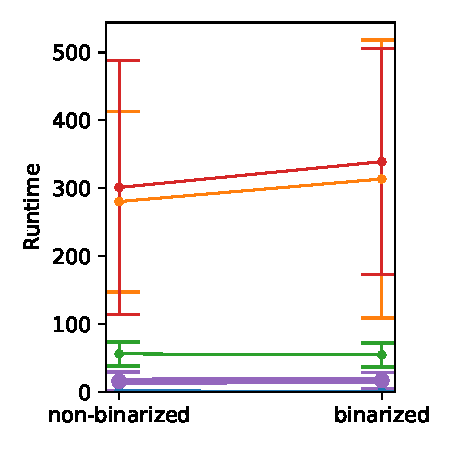
\includegraphics[width=\textwidth]{graphics/eval/runtime_True_1024-1.024_sketchbench.pdf}
    \caption{The average runtime.}
\end{subfigure}
    \begin{subfigure}{.3\textwidth}
    \centering
    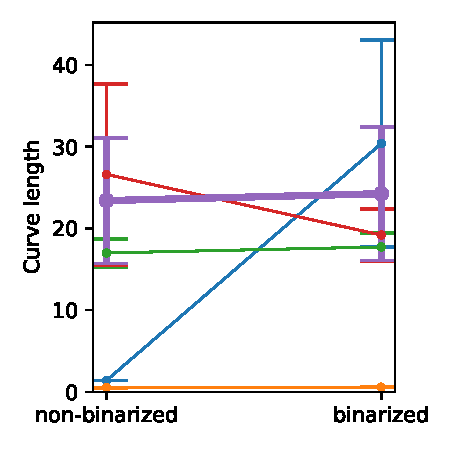
\includegraphics[width=\textwidth]{graphics/eval/curve length_True_1024-1.024_sketchbench.pdf}
    \caption{The average curve length.}
\end{subfigure}
    \begin{subfigure}{.3\textwidth}
    \centering
    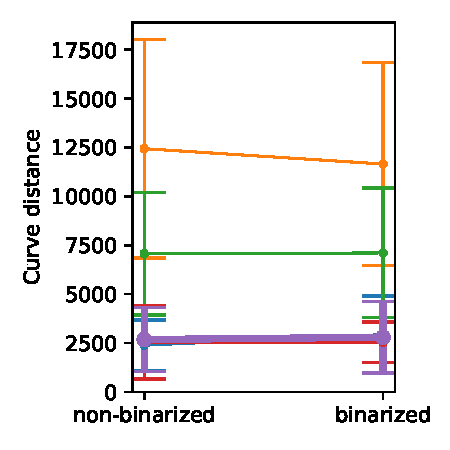
\includegraphics[width=\textwidth]{graphics/eval/curve distance_True_1024-1.024_sketchbench.pdf}
    \caption{The total curve distance.}
\end{subfigure}
    \begin{subfigure}{.3\textwidth}
    \centering
    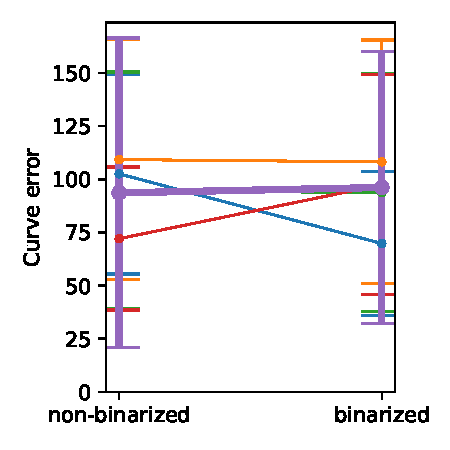
\includegraphics[width=\textwidth]{graphics/eval/curve error_True_1024-1.024_sketchbench.pdf}
    \caption{The average curve error.}
\end{subfigure}
    \caption{The same comparison as in \Cref{fig:metric_True_1024_tonari} on the SketchBench test dataset instead of the Tonari test dataset.}
    \label{fig:metric_True_1024_sketchbench}
\end{figure}

\clearpage
\section{Qualitative Evaluation}

\begin{figure}[h]
    \centering
    \begin{subfigure}{.49\textwidth}
    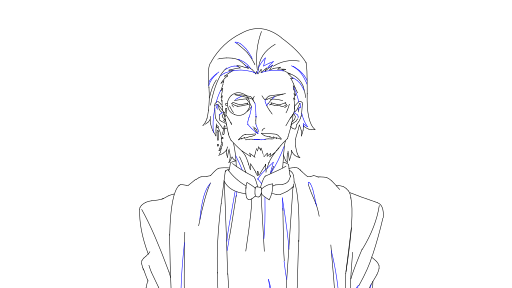
\includegraphics[width=\textwidth]{graphics/outputs/ground-truth/tonari-full_47.png}
    \caption{Input raster image.}
    \end{subfigure}
    \begin{subfigure}{.49\textwidth}
    \includegraphics[width=\textwidth]{graphics/outputs/marked/512-0.512/tonari-full_47.pdf}
    \caption{Output of the developed method.}
    \end{subfigure}
    \begin{subfigure}{.49\textwidth}
    \includegraphics[width=\textwidth]{graphics/outputs/autotrace/binarized/512-0.512/tonari-full_47.pdf}
    \caption{Output of AutoTrace \citep{autotrace}.}
    \end{subfigure}
    \begin{subfigure}{.49\textwidth}
    \includegraphics[width=\textwidth]{graphics/outputs/deepvectechdraw/512-0.512/tonari-full_47.pdf}
    \caption{Output of \citet{DBLP:conf/eccv/EgiazarianVAVST20}.}
    \end{subfigure}
    \begin{subfigure}{.49\textwidth}
    \includegraphics[width=\textwidth]{graphics/outputs/polyvector-flow/binarized/512-0.512/tonari-full_47.pdf}
    \caption{Output of \citet{Puhachov2021KeypointPolyvector}.}
    \end{subfigure}
    \begin{subfigure}{.49\textwidth}
    \includegraphics[width=\textwidth]{graphics/outputs/virtual-sketching/binarized/512-0.512/tonari-full_47.pdf}
    \caption{Output of \citet{mo2021virtualsketching}.}
    \end{subfigure}
    \caption{The output vector image given a Tonari clean animation frame in raster format as input of each line-art image vectorization method studied in this work.}
    \label{fig:tonari-full_47_full_comparison}
\end{figure}


\begin{figure}[h]
    \centering
    \begin{subfigure}{.3\textwidth}
    \includegraphics[width=\textwidth]{graphics/outputs/ground-truth/sketchbench-black_Art_freeform_AP_02_Santiago Rial_norm_cleaned.png}
    \caption{Input raster image of the SketchBench dataset.}
    \end{subfigure}
    \begin{subfigure}{.3\textwidth}
    \includegraphics[width=\textwidth]{graphics/outputs/marked/512-0.512/sketchbench-black_Art_freeform_AP_02_Santiago Rial_norm_cleaned.pdf}
    \caption{Output of the developed method.}
    \end{subfigure}
    \begin{subfigure}{.3\textwidth}
    \includegraphics[width=\textwidth]{graphics/outputs/autotrace/binarized/512-0.512/sketchbench-black_Art_freeform_AP_02_Santiago Rial_norm_cleaned.pdf}
    \caption{Output of AutoTrace \citep{autotrace}.}
    \end{subfigure}
    \begin{subfigure}{.3\textwidth}
    \includegraphics[width=\textwidth]{graphics/outputs/deepvectechdraw/512-0.512/sketchbench-black_Art_freeform_AP_02_Santiago Rial_norm_cleaned.pdf}
    \caption{Output of \citet{DBLP:conf/eccv/EgiazarianVAVST20}.}
    \end{subfigure}
    \begin{subfigure}{.3\textwidth}
    \includegraphics[width=\textwidth]{graphics/outputs/polyvector-flow/binarized/512-0.512/sketchbench-black_Art_freeform_AP_02_Santiago Rial_norm_cleaned.pdf}
    \caption{Output of \citet{Puhachov2021KeypointPolyvector}.}
    \end{subfigure}
    \begin{subfigure}{.3\textwidth}
    \includegraphics[width=\textwidth]{graphics/outputs/virtual-sketching/binarized/512-0.512/sketchbench-black_Art_freeform_AP_02_Santiago Rial_norm_cleaned.pdf}
    \caption{Output of the method by \citet{mo2021virtualsketching}.}
    \end{subfigure}
    \caption{The output vector image given a SketchBench professional sketch in raster format as input of each line-art image vectorization method studied in this work.}
    \label{fig:sketchbench-1.comparison}
\end{figure}

\begin{figure}[h]
    \centering
    \begin{subfigure}{.3\textwidth}
    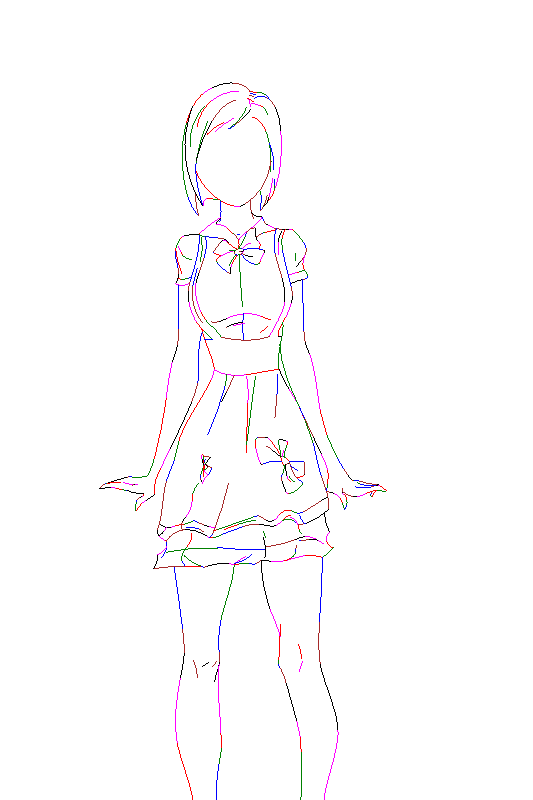
\includegraphics[width=\textwidth]{graphics/outputs/ground-truth/order/sketchbench-black_Art_freeform_AG_03_Branislav Mirkovic_norm_cleaned.pdf}
    \caption{Ground truth vector structure order.}
    \end{subfigure}
    \begin{subfigure}{.3\textwidth}
    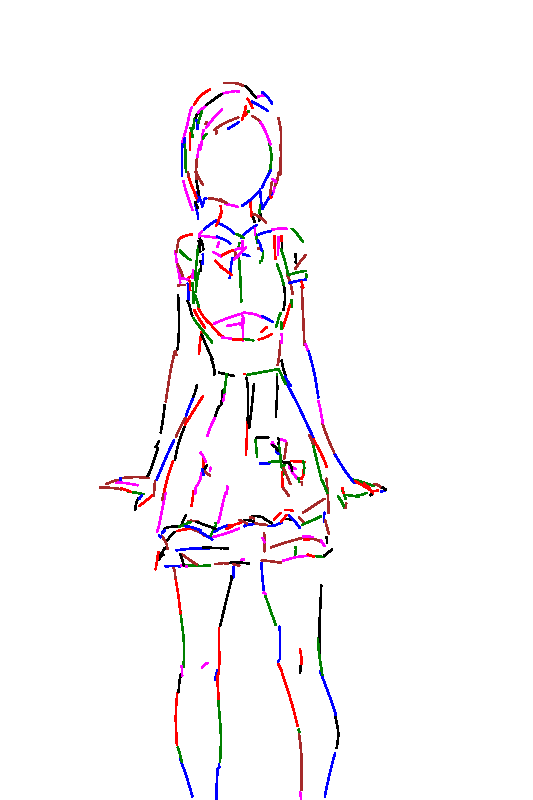
\includegraphics[width=\textwidth]{graphics/outputs/marked/order/sketchbench-black_Art_freeform_AG_03_Branislav Mirkovic_norm_cleaned.pdf}
    \caption{Output of the developed method.}
    \end{subfigure}
    \begin{subfigure}{.3\textwidth}
    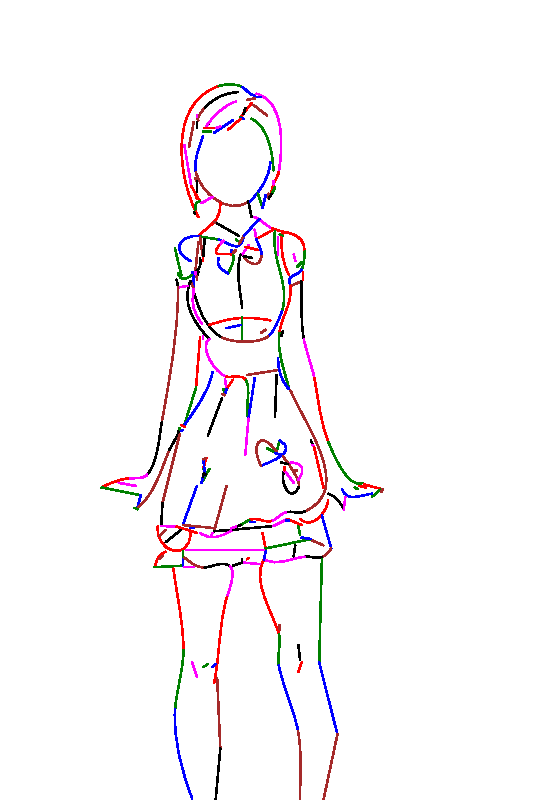
\includegraphics[width=\textwidth]{graphics/outputs/autotrace/order/sketchbench-black_Art_freeform_AG_03_Branislav Mirkovic_norm_cleaned.pdf}
    \caption{Output of AutoTrace \citep{autotrace}.}
    \end{subfigure}
    \begin{subfigure}{.3\textwidth}
    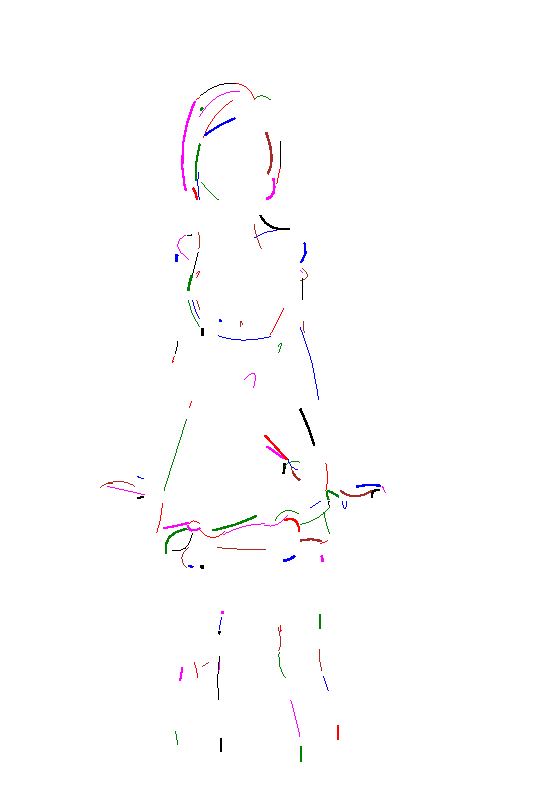
\includegraphics[width=\textwidth]{graphics/outputs/deepvectechdraw/order/sketchbench-black_Art_freeform_AG_03_Branislav Mirkovic_norm_cleaned.pdf}
    \caption{Output of \citet{DBLP:conf/eccv/EgiazarianVAVST20}.}
    \end{subfigure}
    \begin{subfigure}{.3\textwidth}
    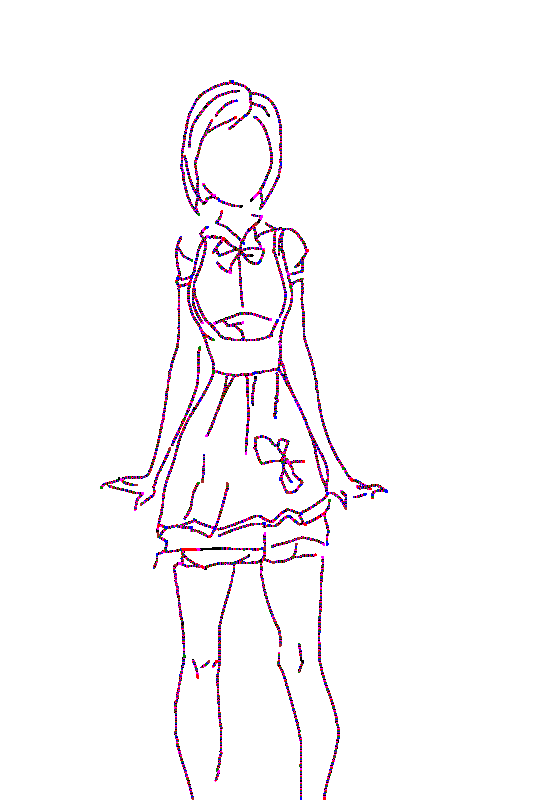
\includegraphics[width=\textwidth]{graphics/outputs/polyvector-flow/order/sketchbench-black_Art_freeform_AG_03_Branislav Mirkovic_norm_cleaned.pdf}
    \caption{Output of \citet{Puhachov2021KeypointPolyvector}.}
    \end{subfigure}
    \begin{subfigure}{.3\textwidth}
    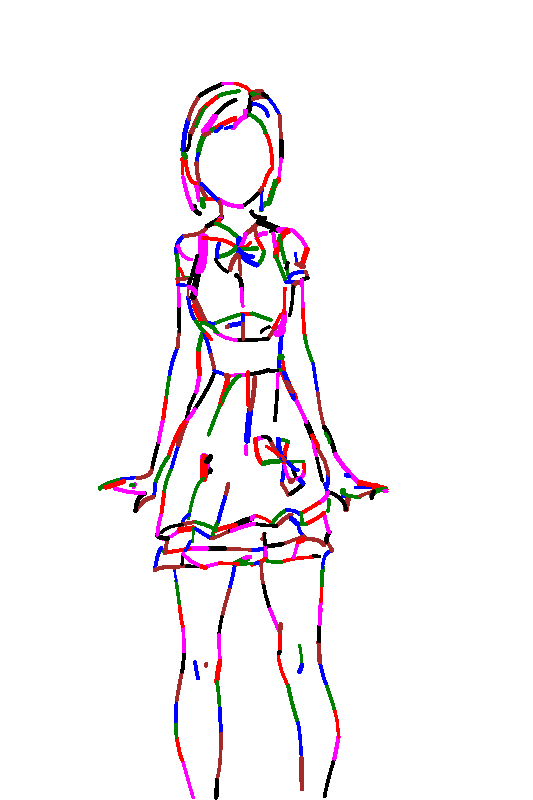
\includegraphics[width=\textwidth]{graphics/outputs/virtual-sketching/order/sketchbench-black_Art_freeform_AG_03_Branislav Mirkovic_norm_cleaned.pdf}
    \caption{Output of the method by \citet{mo2021virtualsketching}.}
    \end{subfigure}
    \caption{The output vector image given a SketchBench professional sketch as input with the vector structure behind the images revealed by representing each curve with a mutually exclusive color.}
    \label{fig:sketchbench-2.order}
\end{figure}